\documentclass[a4paper,9pt]{scrartcl}
\usepackage[utf8]{inputenc}
\usepackage[T1]{fontenc}
\usepackage{xcolor}
\usepackage[yyyymmdd,hhmmss]{datetime}
% \usepackage{subfigure}
\usepackage[top=0.5in, bottom=1in, left=0.4in, right=0.4in]{geometry}
\usepackage{multicol}
\usepackage{subcaption}
\usepackage{graphicx}


\newenvironment{Figure}
  {\par\medskip\noindent\minipage{\linewidth}}
  {\endminipage\par\medskip}

\title{\vspace{-7ex}Analysis of FlexCast Reconfiguration}
\date{\vspace{-10ex}}
\begin{document}
\maketitle


%%%%%%%%%%%%%%%%%%%%%%%%%%%%%%%%%%%%%%%%%%%%%%%%%%%%

\section{Experiment Config.}
\begin{multicols}{3}
    \small
    \begin{itemize}
        \item \textbf{TPCC/AWS Latencies}
        \item \textbf{Exp. Duration:} 2 min
        \item \textbf{Reconfig:} 30 seconds
    \end{itemize}
    \columnbreak
    \begin{itemize}
    	\small
        \item \textbf{Regions/Nodes: 3}  \\(Canada, Sao Paulo, Virginia)
        \item \textbf{Clients: 150} (50 per region)
        \item \textbf{Locality: 95\%}
    \end{itemize}
    \columnbreak
    \begin{Figure}
        \centering
        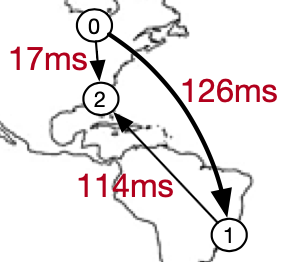
\includegraphics[scale=.29]{figs/CSV}
    \end{Figure}
\end{multicols}

\section{Results}
\small
\begin{multicols}{2}
    \subsection{Throughput}
    \begin{Figure}
        \centering
        
\includegraphics[scale=.6]{exp_reconf/tp/tp.pdf}
    \end{Figure}
    \columnbreak
    \subsection{Latency}
    \begin{Figure}
        \centering
        
\includegraphics[scale=.6]{exp_reconf/latpersec/lat.pdf}
    \end{Figure}
\end{multicols}

\subsection{Reconfiguration details}

\begin{multicols}{2}
    \footnotesize

    \begin{verbatim}
        "workload": [
            {
                "destination": [0, 1],
                "percentage": 0.59979254
            },
            {
                "destination": [0, 2],
                "percentage": 0.032745477
            },
            {
                "destination": [0, 1, 2],
                "percentage": 0.049208425
            },
            {
                "destination": [1, 2],
                "percentage": 0.31825358
            },
        ]
    Took 24 ms 
    \end{verbatim}

    \columnbreak

    \begin{Figure}
        \centering
        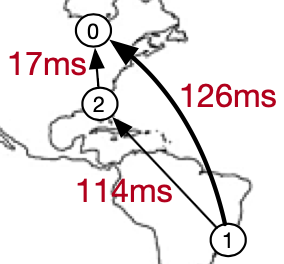
\includegraphics[scale=.3]{figs/SVC.png}
    \end{Figure}

\end{multicols}

\subsection{Latencies per dests (90p)}

\begin{Figure}
    \centering
    
\includegraphics[scale=.6]{exp_reconf/latpersec/perdest/lat[0,1].pdf}
    
\includegraphics[scale=.6]{exp_reconf/latpersec/perdest/lat[0,2].pdf}
    
\includegraphics[scale=.6]{exp_reconf/latpersec/perdest/lat[1,2].pdf}
    
\includegraphics[scale=.6]{exp_reconf/latpersec/perdest/lat[0,1,2].pdf}
\end{Figure}

%%%%%%%%%%%%%%%%%%%%%%%%%%%%%%%%%%%%%%%%%%%%%%%%%%%%

\newpage

\section{Experiment Config.}
\begin{multicols}{3}
    \small
    \begin{itemize}
        \item \textbf{TPCC/AWS Latencies\\ \Large \color{red}NO CLIENT LATENCIES}
        \item \textbf{Exp. Duration:} 2 min
        \item \textbf{Reconfig:} 30 seconds
        \item \Large \color{red} \textbf{GC:} 10 seconds
    \end{itemize}
    \columnbreak
    \begin{itemize}
    	\small
        \item \textbf{Regions/Nodes: 3}  \\(Canada, Sao Paulo, Virginia)
        \item \textbf{Clients: 150} (50 per region)
        \item \textbf{Locality: 95\%}
    \end{itemize}
    \columnbreak
    \begin{Figure}
        \centering
        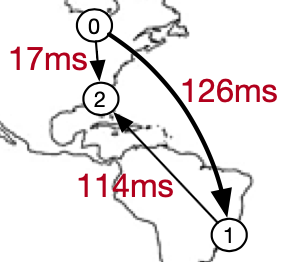
\includegraphics[scale=.29]{figs/CSV}
    \end{Figure}
\end{multicols}

\section{Results}
\small
\begin{multicols}{2}
    \subsection{Throughput}
    \begin{Figure}
        \centering
        
\includegraphics[scale=.6]{noclilat/plots/tp/tp.pdf}
    \end{Figure}
    \columnbreak
    \subsection{Latency}
    \begin{Figure}
        \centering
        
\includegraphics[scale=.6]{noclilat/plots/latpersec/lat.pdf}
    \end{Figure}
\end{multicols}

\subsection{Reconfiguration details}

\begin{multicols}{2}
    \footnotesize

    \begin{verbatim}
        "workload": [
            {
                "destination": [0, 1],
                "percentage": 0.714834
            },
            {
                "destination": [0, 2],
                "percentage": 0.029263614
            },
            {
                "destination": [0, 1, 2],
                "percentage": 0.047801804
            },
            {
                "destination": [1, 2],
                "percentage": 0.2081006
            },
        ]
    Took 22 ms 
    \end{verbatim}

    \columnbreak

    \begin{Figure}
        \centering
        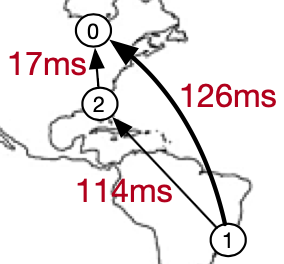
\includegraphics[scale=.3]{figs/SVC.png}
    \end{Figure}

\end{multicols}

\subsection{Latencies per dests (90p)}

\begin{Figure}
    \centering
    
\includegraphics[scale=.6]{noclilat/plots/latpersec/perdest/lat[0,1].pdf}
    
\includegraphics[scale=.6]{noclilat/plots/latpersec/perdest/lat[0,2].pdf}
    
\includegraphics[scale=.6]{noclilat/plots/latpersec/perdest/lat[1,2].pdf}
    
\includegraphics[scale=.6]{noclilat/plots/latpersec/perdest/lat[0,1,2].pdf}
\end{Figure}



%%%%%%%%%%%%%%%%%%%%%%%%%%%%%%%%%%%%%%%%%%%%%%%%%%%%

\newpage

\section{Experiment Config.}
\begin{multicols}{3}
    \small
    \begin{itemize}
        \item \textbf{TPCC/AWS Latencies}
        \item \textbf{Exp. Duration:} 2 min
        \item \textbf{Reconfig:} 30 seconds
        \item \Large \color{red}NO GC
    \end{itemize}
    \columnbreak
    \begin{itemize}
    	\small
        \item \textbf{Regions/Nodes: 3}  \\(Canada, Sao Paulo, Virginia)
        \item \textbf{Clients: 150} (50 per region)
        \item \textbf{Locality: 95\%}
    \end{itemize}
    \columnbreak
    \begin{Figure}
        \centering
        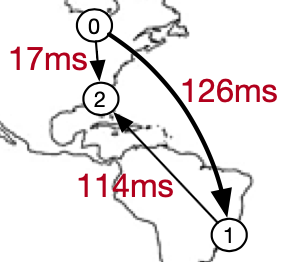
\includegraphics[scale=.29]{figs/CSV}
    \end{Figure}
\end{multicols}

\section{Results}
\small
\begin{multicols}{2}
    \subsection{Throughput}
    \begin{Figure}
        \centering
        
\includegraphics[scale=.6]{exp_reconf/nogc/plots/tp/tp.pdf}
    \end{Figure}
    \columnbreak
    \subsection{Latency}
    \begin{Figure}
        \centering
        
\includegraphics[scale=.6]{exp_reconf/nogc/plots/latpersec/lat.pdf}
    \end{Figure}
\end{multicols}

\subsection{Reconfiguration details}

\begin{multicols}{2}
    \footnotesize

    \begin{verbatim}
        "workload": [
            {
                "destination": [0, 1],
                "percentage": 0.6664093
            },
            {
                "destination": [0, 2],
                "percentage": 0.029835107
            },
            {
                "destination": [0, 1, 2],
                "percentage": 0.05035019
            },
            {
                "destination": [1, 2],
                "percentage": 0.2534054
            },
        ]
    Took 25 ms 
    \end{verbatim}

    \columnbreak

    \begin{Figure}
        \centering
        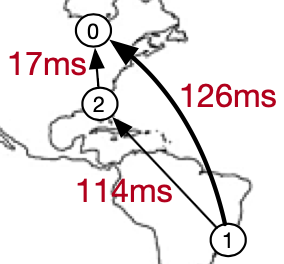
\includegraphics[scale=.3]{figs/SVC.png}
    \end{Figure}

\end{multicols}

\subsection{Latencies per dests (90p)}

\begin{Figure}
    \centering
    
\includegraphics[scale=.6]{exp_reconf/nogc/plots/latpersec/perdest/lat[0,1].pdf}
    
\includegraphics[scale=.6]{exp_reconf/nogc/plots/latpersec/perdest/lat[0,2].pdf}
    
\includegraphics[scale=.6]{exp_reconf/nogc/plots/latpersec/perdest/lat[1,2].pdf}
    
\includegraphics[scale=.6]{exp_reconf/nogc/plots/latpersec/perdest/lat[0,1,2].pdf}
\end{Figure}



%%%%%%%%%%%%%%%%%%%%%%%%%%%%%%%%%%%%%%%%%%%%%%%%%%%%

\newpage

\section{Experiment Config.}
\begin{multicols}{3}
    \small
    \begin{itemize}
        \item \textbf{TPCC/AWS Latencies}
        \item \textbf{Exp. Duration:} 2 min
        \item \textbf{Reconfig:} 30 seconds
        \item \Large \color{red} GC 1 second
    \end{itemize}
    \columnbreak
    \begin{itemize}
    	\small
        \item \textbf{Regions/Nodes: 3}  \\(Canada, Sao Paulo, Virginia)
        \item \textbf{Clients: 150} (50 per region)
        \item \textbf{Locality: 95\%}
    \end{itemize}
    \columnbreak
    \begin{Figure}
        \centering
        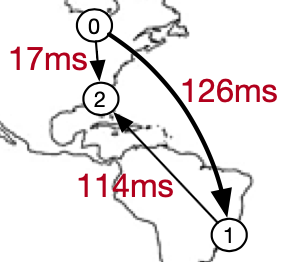
\includegraphics[scale=.29]{figs/CSV}
    \end{Figure}
\end{multicols}

\section{Results}
\small
\begin{multicols}{2}
    \subsection{Throughput}
    \begin{Figure}
        \centering
        
\includegraphics[scale=.6]{exp_reconf/gc1sec/plots/tp/tp.pdf}
    \end{Figure}
    \columnbreak
    \subsection{Latency}
    \begin{Figure}
        \centering
        
\includegraphics[scale=.6]{exp_reconf/gc1sec/plots/latpersec/lat.pdf}
    \end{Figure}
\end{multicols}

\subsection{Reconfiguration details}

\begin{multicols}{2}
    \footnotesize

    \begin{verbatim}
        "workload": [
            {
                "destination": [0, 1],
                "percentage": 0.5822697
            },
            {
                "destination": [0, 2],
                "percentage": 0.031214725
            },
            {
                "destination": [0, 1, 2],
                "percentage": 0.050273508
            },
            {
                "destination": [1, 2],
                "percentage": 0.33624208
            },
        ]
    Took 22 ms 
    \end{verbatim}

    \columnbreak

    \begin{Figure}
        \centering
        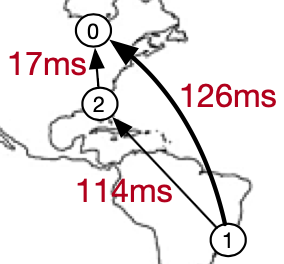
\includegraphics[scale=.3]{figs/SVC.png}
    \end{Figure}

\end{multicols}

\subsection{Latencies per dests (90p)}

\begin{Figure}
    \centering
    
\includegraphics[scale=.6]{exp_reconf/gc1sec/plots/latpersec/perdest/lat[0,1].pdf}
    
\includegraphics[scale=.6]{exp_reconf/gc1sec/plots/latpersec/perdest/lat[0,2].pdf}
    
\includegraphics[scale=.6]{exp_reconf/gc1sec/plots/latpersec/perdest/lat[1,2].pdf}
    
\includegraphics[scale=.6]{exp_reconf/gc1sec/plots/latpersec/perdest/lat[0,1,2].pdf}
\end{Figure}


%%%%%%%%%%%%%%%%%%%%%%%%%%%%%%%%%%%%%%%%%%%%%%%%%%%%

\newpage

\section{Experiment Config.}
\begin{multicols}{3}
    \small
    \begin{itemize}
        \item \textbf{TPCC/AWS Latencies}
        \item \textbf{Exp. Duration:} 2 min
        \item \textbf{Reconfig:} 30 seconds
        \item \Large \color{red} GC 2 second
    \end{itemize}
    \columnbreak
    \begin{itemize}
    	\small
        \item \textbf{Regions/Nodes: 3}  \\(Canada, Sao Paulo, Virginia)
        \item \textbf{Clients: 150} (50 per region)
        \item \textbf{Locality: 95\%}
    \end{itemize}
    \columnbreak
    \begin{Figure}
        \centering
        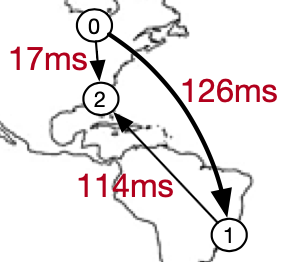
\includegraphics[scale=.29]{figs/CSV}
    \end{Figure}
\end{multicols}

\section{Results}
\small
\begin{multicols}{2}
    \subsection{Throughput}
    \begin{Figure}
        \centering
        
\includegraphics[scale=.6]{exp_reconf/gc2sec/plots/tp/tp.pdf}
    \end{Figure}
    \columnbreak
    \subsection{Latency}
    \begin{Figure}
        \centering
        
\includegraphics[scale=.6]{exp_reconf/gc2sec/plots/latpersec/lat.pdf}
    \end{Figure}
\end{multicols}

\subsection{Reconfiguration details}

\begin{multicols}{2}
    \footnotesize

    \begin{verbatim}
        "workload": [
            {
                "destination": [0, 1],
                "percentage": 0.58594364
            },
            {
                "destination": [0, 2],
                "percentage": 0.03219614
            },
            {
                "destination": [0, 1, 2],
                "percentage": 0.04894861
            },
            {
                "destination": [1, 2],
                "percentage": 0.3329116
            },
        ]
    Took 22 ms 
    \end{verbatim}

    \columnbreak

    \begin{Figure}
        \centering
        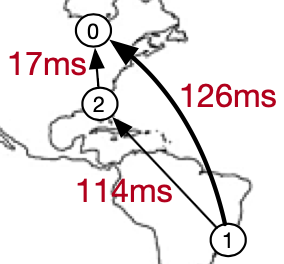
\includegraphics[scale=.3]{figs/SVC.png}
    \end{Figure}

\end{multicols}

\subsection{Latencies per dests (90p)}

\begin{Figure}
    \centering
    
\includegraphics[scale=.6]{exp_reconf/gc2sec/plots/latpersec/perdest/lat[0,1].pdf}
    
\includegraphics[scale=.6]{exp_reconf/gc2sec/plots/latpersec/perdest/lat[0,2].pdf}
    
\includegraphics[scale=.6]{exp_reconf/gc2sec/plots/latpersec/perdest/lat[1,2].pdf}
    
\includegraphics[scale=.6]{exp_reconf/gc2sec/plots/latpersec/perdest/lat[0,1,2].pdf}
\end{Figure}


%%%%%%%%%%%%%%%%%%%%%%%%%%%%%%%%%%%%%%%%%%%%%%%%%%%%

\newpage

\section{Experiment Config.}
\begin{multicols}{3}
    \small
    \begin{itemize}
        \item \textbf{TPCC/AWS Latencies}
        \item \textbf{Exp. Duration:} 2 min
        \item \textbf{Reconfig:} 30 seconds
        \item \Large \color{red} GC 5 seconds
    \end{itemize}
    \columnbreak
    \begin{itemize}
    	\small
        \item \textbf{Regions/Nodes: 3}  \\(Canada, Sao Paulo, Virginia)
        \item \textbf{Clients: 150} (50 per region)
        \item \textbf{Locality: 95\%}
    \end{itemize}
    \columnbreak
    \begin{Figure}
        \centering
        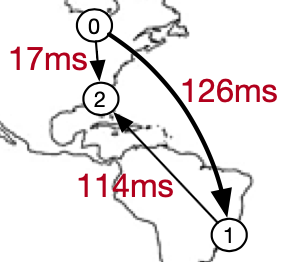
\includegraphics[scale=.29]{figs/CSV}
    \end{Figure}
\end{multicols}

\section{Results}
\small
\begin{multicols}{2}
    \subsection{Throughput}
    \begin{Figure}
        \centering
        
\includegraphics[scale=.6]{exp_reconf/gc5sec/plots/tp/tp.pdf}
    \end{Figure}
    \columnbreak
    \subsection{Latency}
    \begin{Figure}
        \centering
        
\includegraphics[scale=.6]{exp_reconf/gc5sec/plots/latpersec/lat.pdf}
    \end{Figure}
\end{multicols}

\subsection{Reconfiguration details}

\begin{multicols}{2}
    \footnotesize

    \begin{verbatim}
        "workload": [
            {
                "destination": [0, 1],
                "percentage": 0.58656037
            },
            {
                "destination": [0, 2],
                "percentage": 0.03316103
            },
            {
                "destination": [0, 1, 2],
                "percentage": 0.049413003
            },
            {
                "destination": [1, 2],
                "percentage": 0.3308656
            },
        ]
    Took 22 ms 
    \end{verbatim}

    \columnbreak

    \begin{Figure}
        \centering
        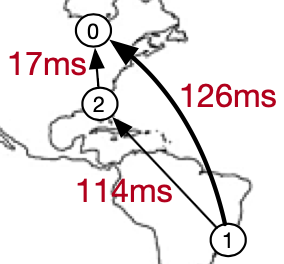
\includegraphics[scale=.3]{figs/SVC.png}
    \end{Figure}

\end{multicols}

\subsection{Latencies per dests (90p)}

\begin{Figure}
    \centering
    
\includegraphics[scale=.6]{exp_reconf/gc5sec/plots/latpersec/perdest/lat[0,1].pdf}
    
\includegraphics[scale=.6]{exp_reconf/gc5sec/plots/latpersec/perdest/lat[0,2].pdf}
    
\includegraphics[scale=.6]{exp_reconf/gc5sec/plots/latpersec/perdest/lat[1,2].pdf}
    
\includegraphics[scale=.6]{exp_reconf/gc5sec/plots/latpersec/perdest/lat[0,1,2].pdf}
\end{Figure}

\newpage

\section{Varying gargbage collection freq}

\subsection{Throughput}

\begin{figure}[ht]
    \begin{subfigure}{.5\textwidth}
        
\includegraphics[width=\textwidth]{gcanalysis/gc0/rc30/clilat/plots/tp/tp.pdf}
        \caption{No GC}
        \label{fig:first}
    \end{subfigure}
    \hfill
    \begin{subfigure}{.5\textwidth}
        
\includegraphics[width=\textwidth]{gcanalysis/gc1000/rc30/clilat/plots/tp/tp.pdf}
        \caption{GC 1 second}
        \label{fig:second}
    \end{subfigure}
    \hfill
    \begin{subfigure}{.5\textwidth}
        
\includegraphics[width=\textwidth]{gcanalysis/gc2000/rc30/clilat/plots/tp/tp.pdf}
        \caption{GC 2 seconds}
        \label{fig:third}
    \end{subfigure}
    \hfill
    \begin{subfigure}{.5\textwidth}
        
\includegraphics[width=\textwidth]{gcanalysis/gc5000/rc30/clilat/plots/tp/tp.pdf}
        \caption{GC 5 seconds}
        \label{fig:third}
    \end{subfigure}
    \hfill
    \begin{subfigure}{.5\textwidth}
        
\includegraphics[width=\textwidth]{gcanalysis/gc10000/rc30/clilat/plots/tp/tp.pdf}
        \caption{GC 10 seconds}
        \label{fig:third}
    \end{subfigure}
            
    \label{fig:figures}
\end{figure}

\newpage

\subsection{Latency}

\begin{figure}[ht]
    \begin{subfigure}{.5\textwidth}
        
\includegraphics[width=\textwidth]{gcanalysis/gc0/rc30/clilat/plots/latpersec/lat.pdf}
        \caption{No GC}
        \label{fig:first}
    \end{subfigure}
    \hfill
    \begin{subfigure}{.5\textwidth}
        
\includegraphics[width=\textwidth]{gcanalysis/gc1000/rc30/clilat/plots/latpersec/lat.pdf}
        \caption{GC 1 second}
        \label{fig:second}
    \end{subfigure}
    \hfill
    \begin{subfigure}{.5\textwidth}
        
\includegraphics[width=\textwidth]{gcanalysis/gc2000/rc30/clilat/plots/latpersec/lat.pdf}
        \caption{GC 2 seconds}
        \label{fig:third}
    \end{subfigure}
    \hfill
    \begin{subfigure}{.5\textwidth}
        
\includegraphics[width=\textwidth]{gcanalysis/gc5000/rc30/clilat/plots/latpersec/lat.pdf}
        \caption{GC 5 seconds}
        \label{fig:third}
    \end{subfigure}
    \hfill
    \begin{subfigure}{.5\textwidth}
        
\includegraphics[width=\textwidth]{gcanalysis/gc10000/rc30/clilat/plots/latpersec/lat.pdf}
        \caption{GC 10 seconds}
        \label{fig:third}
    \end{subfigure}
            
    \label{fig:figures}
\end{figure}


\newpage

\subsection{Volume of acks and notifs}


\begin{figure}[ht]
    \begin{subfigure}{.5\textwidth}
        
\includegraphics[width=\textwidth]{gcanalysis/gc0/rc30/clilat/plots/acksnotifs/acksnotifs.pdf}
        \caption{No GC}
        \label{fig:first}
    \end{subfigure}
    \hfill
    \begin{subfigure}{.5\textwidth}
        
\includegraphics[width=\textwidth]{gcanalysis/gc1000/rc30/clilat/plots/acksnotifs/acksnotifs.pdf}
        \caption{GC 1 second}
        \label{fig:second}
    \end{subfigure}
    \hfill
    \begin{subfigure}{.5\textwidth}
        
\includegraphics[width=\textwidth]{gcanalysis/gc2000/rc30/clilat/plots/acksnotifs/acksnotifs.pdf}
        \caption{GC 2 seconds}
        \label{fig:third}
    \end{subfigure}
    \hfill
    \begin{subfigure}{.5\textwidth}
        
\includegraphics[width=\textwidth]{gcanalysis/gc5000/rc30/clilat/plots/acksnotifs/acksnotifs.pdf}
        \caption{GC 5 seconds}
        \label{fig:third}
    \end{subfigure}
    \hfill
    \begin{subfigure}{.5\textwidth}
        
\includegraphics[width=\textwidth]{gcanalysis/gc10000/rc30/clilat/plots/acksnotifs/acksnotifs.pdf}
        \caption{GC 10 seconds}
        \label{fig:third}
    \end{subfigure}
            
    \label{fig:figures}
\end{figure}


\newpage

\subsection{Size of internal history graph}

\begin{figure}[ht]
    \begin{subfigure}{.5\textwidth}
        
\includegraphics[width=\textwidth]{gcanalysis/gc0/rc30/clilat/plots/acksnotifs/graphsizes.pdf}
        \caption{No GC}
        \label{fig:first}
    \end{subfigure}
    \hfill
    \begin{subfigure}{.5\textwidth}
        
\includegraphics[width=\textwidth]{gcanalysis/gc1000/rc30/clilat/plots/acksnotifs/graphsizes.pdf}
        \caption{GC 1 second}
        \label{fig:second}
    \end{subfigure}
    \hfill
    \begin{subfigure}{.5\textwidth}
        
\includegraphics[width=\textwidth]{gcanalysis/gc2000/rc30/clilat/plots/acksnotifs/graphsizes.pdf}
        \caption{GC 2 seconds}
        \label{fig:third}
    \end{subfigure}
    \hfill
    \begin{subfigure}{.5\textwidth}
        
\includegraphics[width=\textwidth]{gcanalysis/gc5000/rc30/clilat/plots/acksnotifs/graphsizes.pdf}
        \caption{GC 5 seconds}
        \label{fig:third}
    \end{subfigure}
    \hfill
    \begin{subfigure}{.5\textwidth}
        
\includegraphics[width=\textwidth]{gcanalysis/gc10000/rc30/clilat/plots/acksnotifs/graphsizes.pdf}
        \caption{GC 10 seconds}
        \label{fig:third}
    \end{subfigure}
            
    \label{fig:figures}
\end{figure}


\newpage

\subsection{Volume of data in messages}


\begin{figure}[ht]
    \begin{subfigure}{.5\textwidth}
        
\includegraphics[width=\textwidth]{gcanalysis/gc0/rc30/clilat/plots/acksnotifs/volume.pdf}
        \caption{No GC}
        \label{fig:first}
    \end{subfigure}
    \hfill
    \begin{subfigure}{.5\textwidth}
        
\includegraphics[width=\textwidth]{gcanalysis/gc1000/rc30/clilat/plots/acksnotifs/volume.pdf}
        \caption{GC 1 second}
        \label{fig:second}
    \end{subfigure}
    \hfill
    \begin{subfigure}{.5\textwidth}
        
\includegraphics[width=\textwidth]{gcanalysis/gc2000/rc30/clilat/plots/acksnotifs/volume.pdf}
        \caption{GC 2 seconds}
        \label{fig:third}
    \end{subfigure}
    \hfill
    \begin{subfigure}{.5\textwidth}
        
\includegraphics[width=\textwidth]{gcanalysis/gc5000/rc30/clilat/plots/acksnotifs/volume.pdf}
        \caption{GC 5 seconds}
        \label{fig:third}
    \end{subfigure}
    \hfill
    \begin{subfigure}{.5\textwidth}
        
\includegraphics[width=\textwidth]{gcanalysis/gc10000/rc30/clilat/plots/acksnotifs/volume.pdf}
        \caption{GC 10 seconds}
        \label{fig:third}
    \end{subfigure}
            
    \label{fig:figures}
\end{figure}


\newpage

\section{Experiment Config.}
\begin{multicols}{3}
    \small
    \begin{itemize}
        \item \textbf{TPCC/AWS Latencies}
        \item \textbf{Exp. Duration:} 1 min
        \item \textbf{Reconfig:} 10 seconds
        \item \Large \color{red} GC 1 second
    \end{itemize}
    \columnbreak
    \begin{itemize}
    	\small
        \item \textbf{Regions/Nodes: 3}  \\(Canada, Virginia, Sao Paulo)
        \item \textbf{Clients: 150} (50 per region)
        \item \textbf{Locality: 95\%}
    \end{itemize}
    \columnbreak
    \begin{Figure}
        \centering
        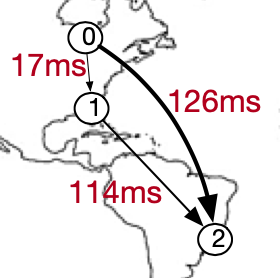
\includegraphics[scale=.29]{figs/CVS.png}
    \end{Figure}
\end{multicols}

\section{Results}
\small
\begin{multicols}{2}
    \subsection{Throughput}
    \begin{Figure}
        \centering
        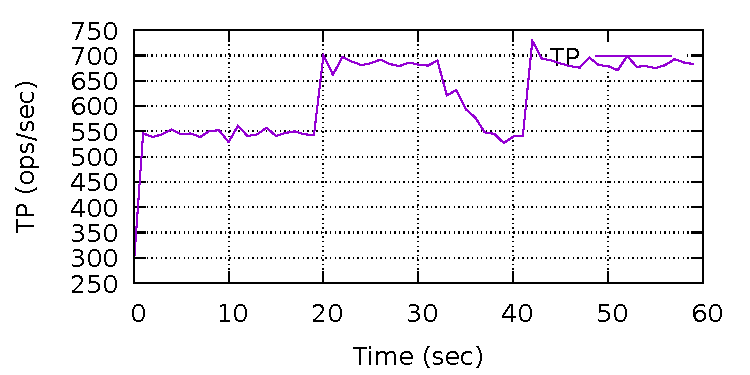
\includegraphics[scale=.6]{chgwload/plots/tp/tp.pdf}
    \end{Figure}
    \columnbreak
    \subsection{Latency}
    \begin{Figure}
        \centering
        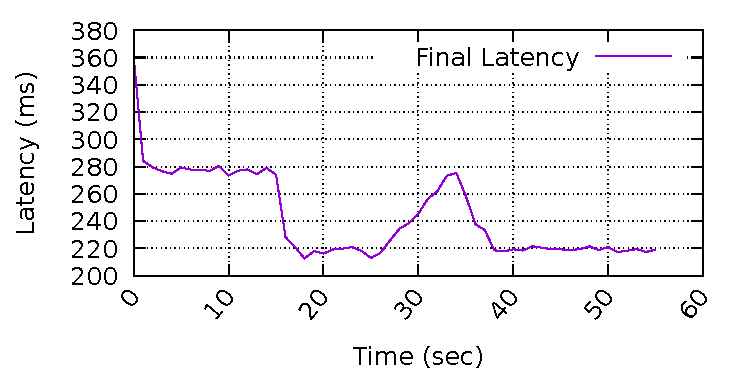
\includegraphics[scale=.6]{chgwload/plots/latpersec/lat.pdf}
    \end{Figure}
\end{multicols}

\subsection{Reconfiguration details}

\begin{multicols}{4}
    \footnotesize

    \begin{verbatim}
        "workload": [
            {
                "destination": [0, 1],
                "percentage": 0.035717566
            },
            {
                "destination": [0, 2],
                "percentage": 0.5288771
            },
            {
                "destination": [0, 1, 2],
                "percentage": 0.04792948
            },
            {
                "destination": [1, 2],
                "percentage": 0.38747588
            },
        ]
    Took 22 ms 
    \end{verbatim}

    \columnbreak

    \begin{Figure}
        \centering
        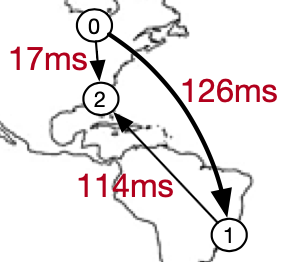
\includegraphics[scale=.3]{figs/CSV.png}
    \end{Figure}

    \columnbreak

    \begin{verbatim}
        "workload": [
            {
                "destination": [0, 1],
                "percentage": 0.031277023
            },
            {
                "destination": [0, 2],
                "percentage": 0.6091093
            },
            {
                "destination": [0, 2, 1],
                "percentage": 0.046555206
            },
            {
                "destination": [2, 1],
                "percentage": 0.3130585
            },
        ]
    Took 22 ms 
    \end{verbatim}

    \columnbreak

    \begin{Figure}
        \centering
        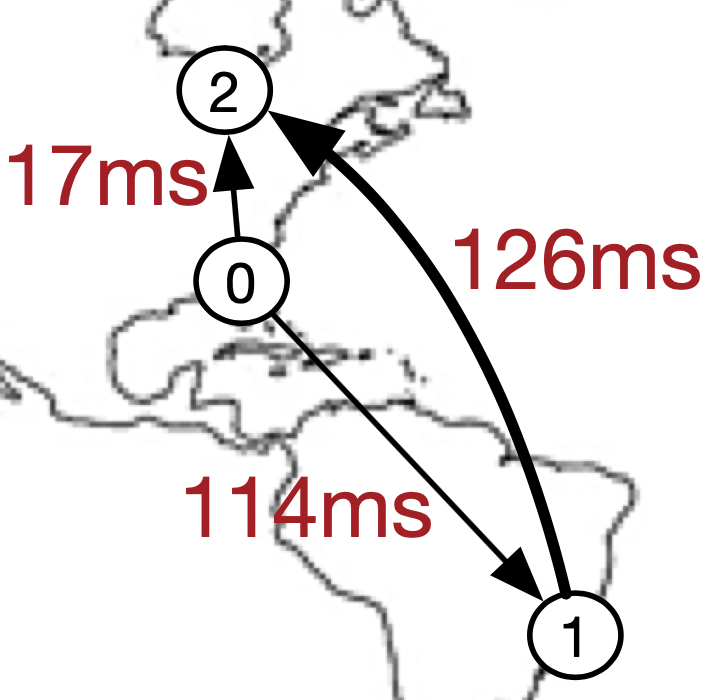
\includegraphics[scale=.3]{figs/VSC_2.png}
    \end{Figure}

\end{multicols}

\subsection{Latencies per dests (90p)}

\begin{Figure}
    \centering
    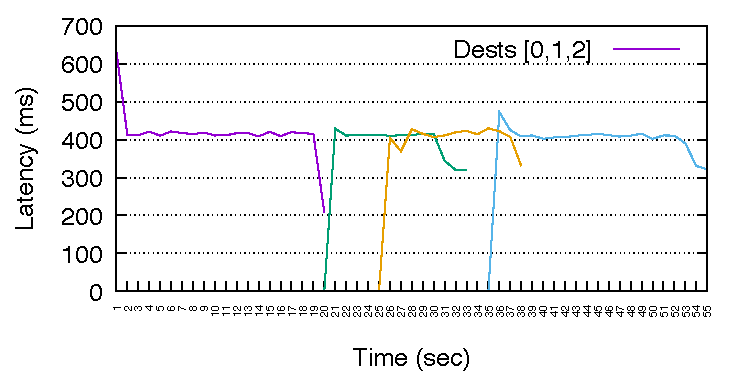
\includegraphics[scale=.6]{chgwload/plots/latpersec/perdest/lat[0,1,2].pdf}
    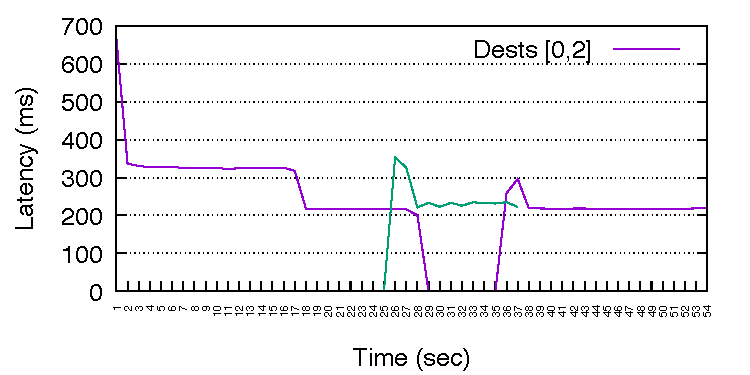
\includegraphics[scale=.6]{chgwload/plots/latpersec/perdest/lat[0,2].pdf}
    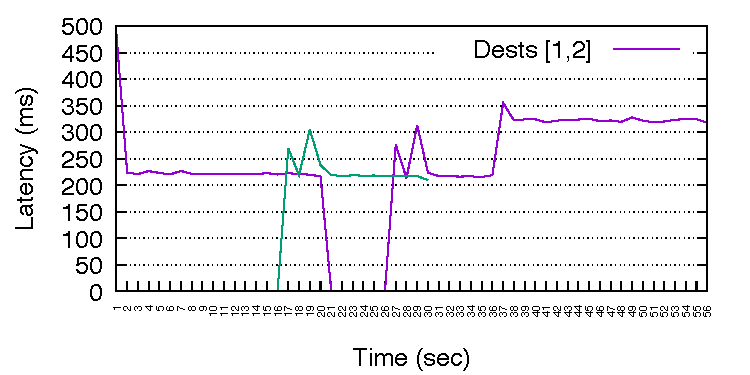
\includegraphics[scale=.6]{chgwload/plots/latpersec/perdest/lat[1,2].pdf}
    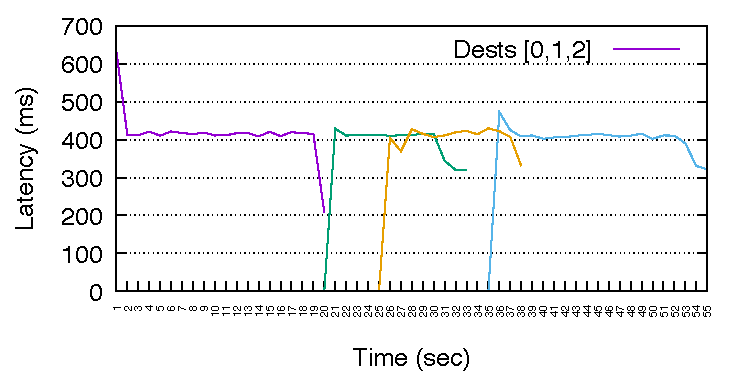
\includegraphics[scale=.6]{chgwload/plots/latpersec/perdest/lat[0,1,2].pdf}
\end{Figure}




\end{document}


